%%%% Proceedings format for most of ACM conferences (with the exceptions listed below) and all ICPS volumes.
\documentclass[sigconf]{acmart}
%%%% As of March 2017, [siggraph] is no longer used. Please use sigconf (above) for SIGGRAPH conferences.

%%%% Proceedings format for SIGPLAN conferences 
% \documentclass[sigplan, anonymous, review]{acmart}

%%%% Proceedings format for SIGCHI conferences
% \documentclass[sigchi, review]{acmart}

%%%% To use the SIGCHI extended abstract template, please visit
% https://www.overleaf.com/read/zzzfqvkmrfzn


\usepackage{booktabs} % For formal tables


% Copyright
%\setcopyright{none}
%\setcopyright{acmcopyright}
%\setcopyright{acmlicensed}
\setcopyright{rightsretained}
%\setcopyright{usgov}
%\setcopyright{usgovmixed}
%\setcopyright{cagov}
%\setcopyright{cagovmixed}


% DOI
\acmDOI{10.475/123_4}

% ISBN
\acmISBN{123-4567-24-567/08/06}

%Conference
\acmConference[GEEKPIE'18]{ACM GeekPie conference}{January 2018}{Zhangjiang, Shanghai China} 
\acmYear{2018}
\copyrightyear{2027}


\acmArticle{4}
\acmPrice{15.00}

% These commands are optional
%\acmBooktitle{Transactions of the ACM Woodstock conference}
\editor{Xiaoyu Song}


\begin{document}
\title{Final Report On Sparse Representation Based Face Recognition}
\titlenote{Produces the permission block, and
  copyright information}
% \subtitle{Extended Abstract}
% \subtitlenote{The full version of the author's guide is available as
%   \texttt{acmart.pdf} document}


\author{Xiaoyu Song}
\author{ID:55958557}
\affiliation{%
  \institution{School of Information Science and Technology, ShanghaiTech University}
}
\email{songxy1@shanghaitech.edu.cn}

\renewcommand{\shortauthors}{X. Song et al.}


\begin{abstract}
This is the final report for SI131 Linear Algebra. This project implement face recognition based on sparse representation. The core of the algorithm is principle components analysis (PCA). This report will demonstrate the procession and results, as well as giving explanations of the details.
\end{abstract}


\keywords{Face Recognition, Computer Vision, Linear Algebra}


\maketitle

\section{Problem Formulation}
When human recognize faces, we actually observe those features that one face's is difference from others'. That's because our faces have so much part similar, but only a little part different which distribute on the 3-dimension outline of our faces. In a 2-dimension picture, this feature is reflected as that there are many areas with almost same value of numbers, and a few areas-which are the outline- with dramatical changes. If two faces have similar those areas, mostly they are from the same person.\\

Hence, out target is to find and sharpen those areas. An image can be understand by the computer as a matrix. We know that for data partly with relationships, they may look complicated in one coordinate system, but look simple and clear in other coordinate systems. In the later systems, we can easily abandon some data less useful and concentrate on the important data. In this case, the data areas that everyone is similar in are right the less important data. We can find and exclusive them by express the picture in another system, also known as basis transformation.\\

Using basis transformation to extract the important components, this is called principle components analysis (PCA). In mathematics, this can be implemented by finding the covariance matrix of centralized origin matrix, and then the eigenvectors of the covariance matrix whose corresponded eigenvalue are the biggest ones are the principle components bases. Using this bases to represent the imagines, and the difference between different people's will be clear and it will be easy to recognize the test face.\\

The formulation is shown below:\\

Read the training samples as vectors:
\begin{displaymath}
	x_i: i = 1, 2, 3, 4,\cdots, m
\end{displaymath}

Calculate the mean:
\begin{displaymath}
	\mu = \frac{\sum_{i=1}^{m}x_i}{m}
\end{displaymath}

Centralize:
\begin{displaymath}
	\phi_i = x_i - \mu
\end{displaymath}

Calculate the covariance matrix:
\begin{displaymath}
	C = \frac{\sum_{i=1}^m\phi_i\phi_i^{T}}{m} = AA^{T}
\end{displaymath}

where
\begin{displaymath}
	A = [\phi_1, \phi_2, \cdots, \phi_{m}]
\end{displaymath}

Calculate the eigenvectors $v_i$ and their corresponding eigenvalues $\lambda_i$ of $C$ and combined as column vectors sorted in descending order. Taking the first $k$ vectors as the principle component, which is
\begin{displaymath}
	E = [v_1, v_2,\cdots,v_k]
\end{displaymath}

and satisfying
\begin{displaymath}
	\frac{\sum_{i=1}^k\lambda_i}{\sum_{i}\lambda_i} \ge 95%
\end{displaymath}

Project the images of training samples onto the eigen-subspace, 
\begin{displaymath}
	P = E'X = E'[x_1, x_2,\cdots, x_n]
\end{displaymath}

For test images, take the same steps as above and project it on the eigen-subspace, then find the nearest component in the stan- dard matrix by minimizing the error with con- straint of one-norm of x:
\begin{displaymath}
	||y - Px||_2^2 + \lambda||x||_1
\end{displaymath}
\section{Algorithm}

The Algorithm is mainly comprised of the following steps:\\

	1.read the training set\\
    
	2.construct matrix and transpose to X\\
    
	-----------------------call PCA--------------------------\\
    
	3.find the covariance matrix\\
    
	4.calculate the eigenvectors COEFF and eigenvalues LATENT\\
    
	-----------------------PCA ends--------------------------\\
    
	5.take k eigenvectors with 95\% proportion as E\\
    
	6.project training matrix and test matrix on E\\
    
    7.find the most possible faces and calculate the accuracy\\
    
\section{Improvements}

To make the function perform faster and better, I add the following improvements:\\

	1.Regularization.\\
    
    After reading the images in, firstly regularize the matrix ti make the elements are double and in the range of [0, 1]. This makes the calculations easier.\\
    
    2.Resize the picture before transformations.\\
    
    The resize is constant proportional. I set a resize coefficient as a parameter. This may make the function faster with higher accuracy.\\
    
    3.Exclude the ambient.\\
    
    The image with name 'Ambient' in every folder is the ambient light in the environment. Minus each picture with resized and reshaped ambient reduce the noise from the environment and may make the performance better.\\
    
\section{Dataset Description}

The dataset is uniform with light, middle and dark lights, so any bias will make the algorithm work badly in other areas. To avoid overfitting, I randomly choose training set, validation set and test set. And I make sure that the validation set is small than the test set, with a proportion at about $1/4$.\\

\section{Performance}

In this project, I mostly focus on three parameters: the coefficient $\lambda$, the size of training set numTrainee, and the parameter set by myself-the proportion of the resize.\\

Since the numTrainee is the most user-decided parameter, I consist it on 5 and first find the possible best range of $\lambda$.

\begin{center}
	\begin{tabular}{cccc}
	\hline
	$\lambda$& 1st& 2nd& avg\\
	\hline
	0& 0.7068& 0.7068& 0.7068\\
	0.000076& 0.8064& 0.8102& 0.8083\\
	0.5& 0.8064& 0.8064& 0.8064\\
	1& 0.8026& 0.7951& 0.79885\\
	1.5& 0.8195& 0.7744& 0.79695\\
	2& 0.8120& 0.9045& 0.85825\\
	2.5& 0.8120& 0.7801& 0.79605\\
	\hline
	\end{tabular}
\end{center}

\begin{figure}
    \centering
    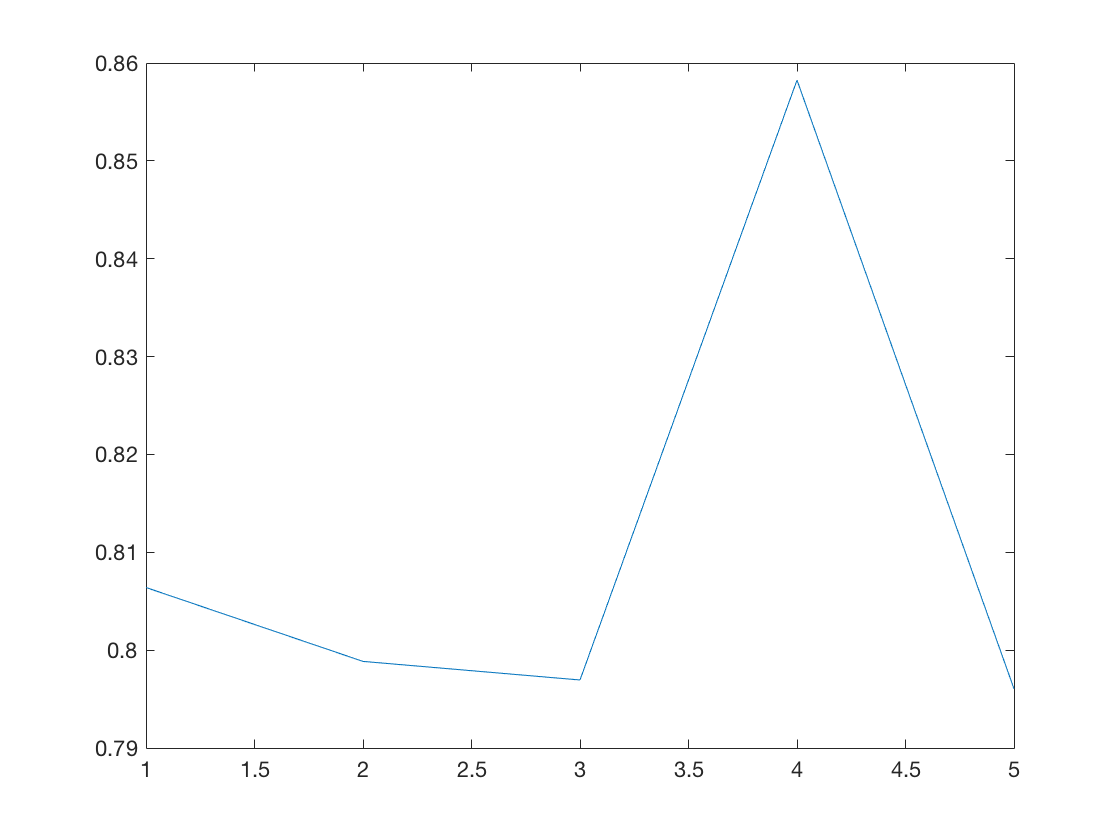
\includegraphics[width=0.9\columnwidth]{lambda.png}
    \caption{Fig.1. The $\lambda$ range}
\end{figure}

From this table and picture we can see that when $\lambda$ is around 2, it reaches a peak.\\

That give us a range to find when $\lambda$ is best. Before that, we can just take $\lambda = 2$ and find the best resize.\\

\begin{center}
	\begin{tabular}{cccc}
	\hline
	resize& 1st& 2nd& avg\\
	\hline
	1.0& 0.8120& 0.7763& 0.79415\\
	0.9& 0.8083& 0.8064& 0.80735\\
	0.8& 0.8064& 0.8008& 0.8036\\
	0.7& 0.7763& 0.8139& 0.7951\\
	0.6& 0.8008& 0.7801& 0.79045\\
	0.5& 0.7726& 0.7726& 0.7726\\
	\hline
	\end{tabular}
\end{center}

\begin{figure}
    \centering
    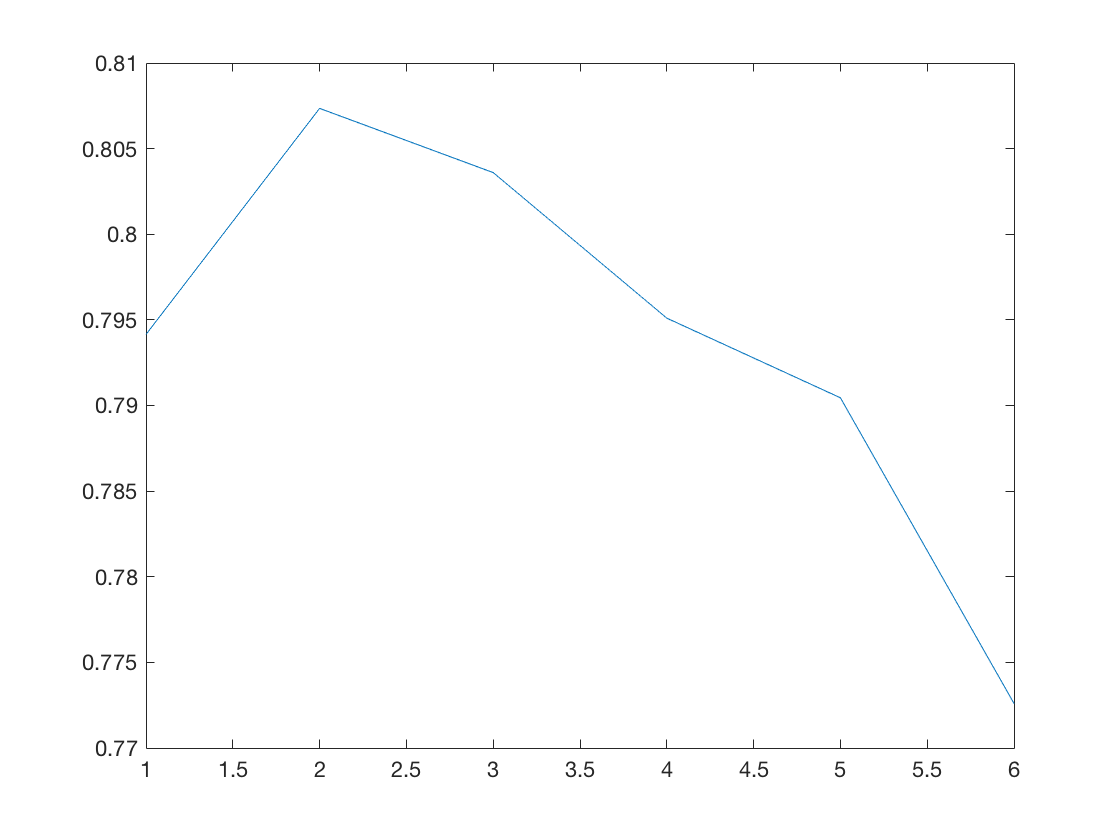
\includegraphics[width=0.9\columnwidth]{resize.png}
    \caption{Fig.1. The resize value}
\end{figure}

As shown above, when resize is 0.9, the accuracy is best.\\

Look back to $\lambda$ and numTrainee.\\


\begin{center}
	\begin{tabular}{cccccc}
	\hline
numTrainee|$\lambda$&	1.6&	 1.8&	2&	2.2&	 2.4\\
	\hline
5&	0.8008&	0.8139&	0.8327&	0.8217&	0.7763\\
5&	0.7632&	0.7876&	0.7857&	0.8008&	0.7820\\
10&	0.8381&	0.8259&	0.8644&	0.8603&	0.8563\\
10&	0.8441&	0.8765&	0.8462&	0.8421&	0.8603\\
15&	0.8772&	0.8860&	0.8553&	0.8596&	0.8684\\
15&	0.8531&	0.8640&	0.8618&	0.8662&	0.8618\\
20&	0.8708&	0.8684&	0.8565&	0.8684&	0.8684\\
20&	0.8732&	0.8756&	0.8828&	0.8684&	0.8732\\
25&	0.8480&	0.8626&	0.8596&	0.8713&	0.8509\\
25&	0.8655&	0.8480&	0.8626&	0.8626&	0.8713\\
30&	0.8618&	0.8520&	0.8421&	0.8538&	0.8388\\
30&	0.8421&	0.8618&	0.8454&	0.8388&	0.8553\\
35&	0.8496&	0.8308&	0.8383&	0.8346&	0.8346\\
35&	0.8271&	0.8383&	0.8383&	0.8195&	0.8271\\
	\hline
	\end{tabular}
	numTrainee v.s. $\lambda$
\end{center}



\begin{center}
	\begin{tabular}{cccccc}
	\hline
numTrainee|$\lambda$&	1.6&	 1.8&	2&	2.2&	 2.4\\
	\hline

5&	0.782&	0.80075&	0.8092&	0.81125&	0.77915\\
10&	0.8411&	0.8512&	0.8553&	0.8512&	0.8583\\
15&	0.86515&	0.8750&	0.85855&	0.8629&	0.8651\\
20&	0.872&	0.872&	0.86965&	0.8684&	0.8708\\
25&	0.85675&	0.8553&	0.8611&	0.86695&	0.8611\\
30&	0.85195&	0.8569&	0.84375&	0.8463&	0.84705\\
35&	0.83835&	0.83455&	0.8383&	0.82705&	0.83085\\

	\hline
	\end{tabular}
	average numTrainee v.s. $\lambda$
\end{center}

From above we know, when the numTrainee is in [15, 20] and $\lambda$ is around [1.6, 1.8], the accuracy is the highest.\\

In the function, I choose $\lambda = 1.75$ and resize$ = 0.9$.


\section{Observation}



The performance is not very good.\\

First the speed is not quick enough, and this may be improved by changing the method of PCA-experiments show that the operation of big matrix is the main cause for low speed. SVD may work better, but the ultimate method is to find a way to avoid big matrix operation. \\

Since in PCA, score and the whole covariance are not essential, we only need the first some eigenvectors, so we do not need to calculate the whole covariance matrix and then find the whole eigenvector matrix. There is a 'approximate matrix' method which can solve the first k eigenvector problem.\\

Second, the accuracy is also not satisfying. A good way to improve it is to change the way of finding the best-match image. We can use other functions or constraint equations (mean not gradient descent) or we can change the method of confirming the right person(mean not by find the largest coefficients sum).\\

Third, there are more parameters that can be adjust. This makes the function serves better.
\section{Acknowledgement}

I would like to express my gratitude to our TA Ding Peng, and my classmate Zeng Xiangyu. The two respectable men answered my questions patiently and give me useful directions.\\

\bibliographystyle{ACM-Reference-Format}
\bibliography{reference} 


\end{document}
